\chapter{Empirical evaluation}
% \label{ch:evaluation}

% Chapter Introduction
% - set up the scene
% - state what is the aim of the evaluation (accuracy of the parser to segment text, 
% assign unit classes, element functions and systemic features to text segments)
% - explain how that aim is achieved (compare the segmentation, element assignment, 
% feature assignment available in the corpus with that coming from the parser)
% - how the chapter is structured  
% Main sections
% - describe the corpora
%   (provenance, annotations, size metrics, quality assessment; data examples ?)
% - describe the method of comparing parser output to corpus annotations 
% - present the evaluation data for: Mood and Transitivity elements + unit classes 
%   (focus on constituent identification)
% - present the evaluation data for: Mood and Transitivity features 
%   (focus on feature accuracy per system for the identified units)
% - *interpret evaluation data and present findings
%   (or should this be provided when each evaluation data is presented) 
% Conclusions
% - concise summary of the main findings


    This chapter aims to evaluate the Parsimonious Vole parser accuracy at generating text analysis in general; and how well it performs at unit boundary detection (i.e text segmentation), unit class assignment, element assignment and feature selections in particular. The grammar that is employed in this evaluation was introduced in Chapter \ref{ch:the-grammar} and the corpus will be introduced in Section \ref{sec:corpus}. 
    
    The evaluation data are collected by comparing the labelled segments  available in the corpus to the labelled segments in the parser output. The main measurements of parser accuracy considered here are \textit{precision} and \textit{recall} and $F_1$ scores. The parser \textit{precision} measures how many segments have been produced by the parser that are also found in manual analysis; and the parser \textit{recall} measures how many correct segments have been produced by the parser relative to the total number of produced segments. $F_1$ score is a harmonic mean of the precision and recall.
    
    The corpus used in this evaluation do not constitute a true gold standard and there are, due to different reasons, some differences to the parser. These differences will be described in detail in Section \ref{sec:differences}.
    
    The evaluation methodology, which will be described in detail in Section \ref{sec:evaluation-methodology}, considers perfect alignment between segment boundaries and their labels, and also considers partial alignment of segments with the same label. This means that segments such as the ones in Listings \ref{lst:exampleText1} and \ref{lst:exampleText1} are given some credit in the alignment process.

\noindent
\begin{minipage}{\linewidth}
\begin{lstlisting}[numbers=left,basicstyle=\small\tt, stepnumber=1,firstnumber=0,frame=single,caption=Example segment from the corpus,label=lst:exampleText1,escapeinside={(*}{*)}]
(*\textcolor{black!50}{$_{587}$}*)forced me into treatment(*\textcolor{black!50}{$_{611}$}*)
\end{lstlisting}
\end{minipage}

\noindent
\begin{minipage}{\linewidth}
\begin{lstlisting}[numbers=left,basicstyle=\small\tt, stepnumber=1,firstnumber=0,frame=single,caption=Example segment from the parser output,label=lst:exampleText2,escapeinside={(*}{*)}]
(*\textcolor{black!50}{$_{583}$}*)and forced me into treatment .(*\textcolor{black!50}{$_{612}$}*)
\end{lstlisting}
\end{minipage}    
     

\section{Evaluation corpus}
\label{sec:corpus}
% (provenance, annotations, size metrics, quality assessment; data examples ?)
    
    \begin{table}[!ht]
        \centering
        \resizebox{\textwidth}{!}{%
        \begin{tabular}{|c|c|c|c|c|c|}
            \hline
            \textbf{Corpus name} & \textbf{Meta-function} & \textbf{\begin{tabular}[c]{@{}c@{}}\# characters\\ (thousands)\end{tabular}} & \textbf{\# clauses} & \textbf{Annotator(s)}         \\ \hline
            OCD            & Mood            & 16.2                                                                         & 147                 &  Ela Oren \& Eugeniu Costetchi \\ \hline
            OE1         & Transitivity         & 51.8                                                                         & 1503                & Anke Schultz                  \\ \hline
            % BTC             & Transitivity         & 5.6                                                                          & 157                 & Anke Schultz                  \\ \hline
        \end{tabular}
        }
        \caption{Evaluation corpus summary}
        \label{tab:corpus-sumary}
    \end{table}
    
    % TODO: introduce corpora
    
    % The OE1 corpus was not developed for the purpose of evaluating constituency in the current parser. Nevertheless the provided segmentation however can be used to evaluate the boundaries of constituent segments. This corpus are primitively used for evaluation of the constituent's semantic function and some TRANSITIVITY features (to the degree provided in the corpus). To enable each of these evaluations the annotation data and parser output needed to be uniformly represented in order to be in alignment with the parser output. To achieve this, feature names were harmonised with the ones from PTDB following the same adjustments as described in Section \ref{sec:claning-ptdb}. In Section \ref{sec:results},  the empirical findings of the current evaluation are described.

\subsection{OE1 corpus}

    The Bremen Translation Corpus (BTC) was created at the University of Bremen by Kerstin Fischer, Anatol Stefanowitsch and Anke Schulz. It consists of comparable and parallel texts. The comparable part consists of a series of newsgroup texts of about 10,000 words of English text and another 10,000 words of German, text taken from the same register. The parallel part, called EDNA, is much larger comprising about 100,000 words of parallel English-German text. Anke uses in her thesis 10,000 words of parallel text and about the same of comparable text \citep[31]{schulz2015me}. In this evaluation only the English part is considered that comprises 31 files spanning over 1503 clauses and 20864 words. In addition, Anke provided a set of similarly annotations of the ``Little Red Riding Hood'' fairy tale comprising 157 clauses that is also included into this evaluation as part of OE1. 
    
    The corpus annotations cover Cardiff TRANSITIVITY, THEME and MODIFICATION system networks. The grammatical details and the annotation methodology are covered in detail in \citet{schulz2015me}.

\subsection{OCD corpus}

     The first corpus (OCD) was created by Ela Oren and myself and is focused on syntactic constituency structure and clause MOOD features. The texts represent blog articles of people diagnosed with Obsessive Compulsive Disorder (OCD) who self-report on the challenge of overcoming OCD. The corpus contains four texts comprising all together 988 clauses and 8605 words. 

\subsection{Differences between the corpus annotation and parser output}
\label{sec:differences}
% todo rename section

% todo: introduce this example
\begin{minipage}{\linewidth}
\begin{lstlisting}[numbers=left,basicstyle=\small\tt, stepnumber=1,firstnumber=0,frame=single,caption=Raw text example in annotation data,label=lst:exampleText,escapeinside={(*}{*)}]
(*\textcolor{black!50}{$_{0}$}*)Red riding hood excerpt(*\textcolor{black!50}{$_{24}$}*)
(*\textcolor{black!50}{$_{25}$}*)"What have you in that basket,   Little Red Riding Hood?"(*\textcolor{black!50}{$_{82}$}*)
(*\textcolor{black!50}{$_{83}$}*)
(*\textcolor{black!50}{$_{84}$}*)"Eggs and butter and cake, Mr. Wolf."(*\textcolor{black!50}{$_{111}$}*)
\end{lstlisting}
\end{minipage}

    Listing \ref{lst:exampleText} presents an example raw text from the annotation dataset containing an initial title line and two sentences separated by an empty line. The greyed index numbers at the beginning and end of each line indicate character offsets. In BTC corpus files, the first line plays the role of a header containing the title or the file name. In this example it is a title. Either way, this first line is neither considered for annotation nor parsing. 
    
    In the OCD file the text was not normalised before the annotation started. Mostly it is organised as one sentence per line, but there are instances of  extra blank lines or several some sentences per line as one continuous block. The text may also sporadically contain tabs and blank spaces such as here in line 1 between the comma and the ``Little Red Riding Hood''. 

    It is noteworthy to mention that there are segmentation errors in a few cases from the OCD corpus. Some segments are either shifted and include the adjacent spaces (e.g. `` getting this push'' instead of ``getting this push'') or, the converse, leave out one or two characters of a marginal word (e.g. ``the balanc'' instead of ``the balance''). Such 

    The parser diverges in a few ways from the corpus annotation methodology when it comes to punctuation marks and treatment of conjunctions. 
    
    In the corpus, punctuation marks such as commas, semicolons, three dots and full stops are not included in the constituent segments while the parser includes them at the end of each adjacent segment. 
    
    The treatment of conjunctions that was discussed in Section \ref{sec:coordination} differs as well. In the corpus, the conjunctions (such as ``and'', ``but'', ``so'', etc.) are excluded from the conjunct segments; they are considered markers in the clause/group complexes rather than part of the constituent. The parser, on the other hand, includes the conjunctions in the following adjacent segment. For example in the corpus there we find segment ``forced me into treatment'' while the parser produces a slightly larger segment ``and forced me into treatment.'' that includes the conjunction at the beginning and the full-stop at the end.
    
    Moreover the conjunct segment spans differ as well due to difference in treatment. Instead of being analysed in parallel, having sibling status as depicted in Figure \ref{fig:segment-conjunction-paralel}, the parse generated conjunct segments are subsumed in a cascade from the former to the latter as depicted in Figure \ref{fig:segment-conjunction-subsumed}.

    \begin{figure}[!ht]
        \centering
        \begin{subfigure}[b]{0.47\textwidth}
            \centering
            \begin{tikzpicture}[pattern-node]
            \node[pattern-node] (start) {};
            \node[pattern-node, right = 5em of start] (end) {};
            \draw[edge-style] (start) -- (end) node[midway, above]{conjunct 1};
            
            \node[pattern-node, right = .5em of end] (conj) {and};
            
            \node[pattern-node, right = .5em of conj] (start1) {};
            \node[pattern-node, right = 5em of start1] (end1) {};
            \draw[edge-style] (start1) -- (end1) node[midway, above]{conjunct 2};
            
            \end{tikzpicture}
            \caption{Conjuncts annotated as parallel segments}
            \label{fig:segment-conjunction-paralel}
        \end{subfigure}
        \quad
        \begin{subfigure}[b]{0.47\textwidth}
            \centering
            \begin{tikzpicture}[pattern-node] 
            \node[pattern-node] (start) {};
            \node[pattern-node, right =14em of start] (end) {};
            \draw[edge-style] (start) -- (end) node[midway, above]{conjunct 1};
            
            
            \node[pattern-node, below = 0.1em of end] (end1) {};
            \node[pattern-node, left = 8em of end1] (start1) {};
            \draw[edge-style] (start1) -- (end1) node[midway, above]{conjunct 2};
            
            \node[pattern-node, below = -0.6em of start1, xshift=1.8em] (conj) {and};        
            \end{tikzpicture}
            \caption{Conjuncts annotated as subsumed segments}
            \label{fig:segment-conjunction-subsumed}
        \end{subfigure}
        \caption{Treatment of conjunctions in the corpus compared to the parser}
        \label{fig:conjunction-treatment}
    \end{figure}

    % TODO: argue why partial match is valuable 

\section{Evaluation methodology}
\label{sec:evaluation-methodology}

\subsection{Segments}

    To compare the segment boundaries we need to understand how they are represented in each output and how they can be brought to a common form comparison. 
    All datasets were created with the UAM Corpus Tool \citep{ODonnell2008,ODonnell2008a} version 2.4. The annotations, in this software, are recorded as segments spanning from a start to an end position in the text file together with the set of features (selected from a systemic network) attributed to that segment. There are no constituency or dependency relations between segments. The XML representation of an example annotation segment is provided in Listing \ref{lst:segment1}. There the \textit{id} attribute indicates the unique identification number within the annotation dataset, the \textit{start} and \textit{end} attributes define the segment between two character offsets relative to the beginning of the text file.

\begin{minipage}{\linewidth}
\begin{lstlisting}[language=XML,basicstyle=\small\tt,frame=single,caption=Segment example in UAM corpus tool,label=lst:segment1]
<segment id="4" start="20" end="27" 
features="configuration;relational;attributive" 
state="active"/>
\end{lstlisting}
\end{minipage}

     In the current evaluation, the segments are reduced to carry only one label. The consequence is that segments with multiple features (Figure \ref{fig:segment-multiple}) are broken down into multiple segments with the same span (Figure \ref{fig:segment-simple}) for each feature. When each segment contains exactly one feature the evaluation can be focused on one or a set of features of interest by selecting only the segments that contain exactly those. 

    \begin{figure}[!ht]
        \centering
        \begin{subfigure}[b]{0.47\textwidth}
            \centering
            \begin{tikzpicture}[pattern-node]
            \node[pattern-node] (start) {20};
            \node[pattern-node, right = 7em of start] (end) {27};
            \draw[edge-style] (start) -- (end) node[midway, above]{configuration,\\relational,\\attributive};
            \end{tikzpicture}
            \caption{A segment with a set of features}
            \label{fig:segment-multiple}
        \end{subfigure}
        \begin{subfigure}[b]{0.47\textwidth}
            \centering
            \begin{tikzpicture}[pattern-node] 
            \node[pattern-node] (start1) {20};
            \node[pattern-node, right = 7em of start1] (end1) {27};
            \draw[edge-style] (start1) -- (end1) node[midway, above]{configuration};
            
            \node[pattern-node, below = 1em of start1] (start2) {20};
            \node[pattern-node, right = 7em of start2] (end2) {27};
            \draw[edge-style] (start2) -- (end2) node[midway, above]{relational};
            
            \node[pattern-node, below = 1em of start2] (start3) {20};
            \node[pattern-node, right = 7em of start3] (end3) {27};
            \draw[edge-style] (start3) -- (end3) node[midway, above]{attributive};	
            \end{tikzpicture}
            \caption{A set of segments with single features}
            \label{fig:segment-simple}
        \end{subfigure}
        \caption{Example of breaking down a segment with multiple features into set of segments with a single feature}
        \label{fig:segment-breackdown}
    \end{figure}

% todo conclude the section 

\subsection{reading the corpus segments as a set of mono labelled segments}


\subsection{Turning parser output into a set of mono labelled segments}
% todo update the section start
    
    In order to compare the parser generated output to the corpus segments they need to be turned into the same form. In this section I describe the task of turning rich constituency graphs (CG) into labelled segments similar to those in the corpus. 
    
    Once the parser receives a text as an input, it normalises and segments the text first before performing anything else. Corpus annotation is performed on the raw non-normalised text. To make the parser output segments comparable to the ones in the corpus they need to refer, in terms of their offsets and indexes, to the same raw text. Before the evaluation can take place the parser output segments need to be re-indexed to correspond to the input raw text. 
    %This sections explains the process how the output segmentation is remapped onto the original text.
    
    To fulfil this task, the text processed by the parser is re-indexed back into the original raw text at the level of words (tokens), constituents and sentences. Algorithm \ref{alg:re-index-text} provides pseudo-code of the indexing process.

    \begin{algorithm}[!ht]
        \Input {CG bundle, \text} %, \dg
        \Begin {
            offset $\leftarrow$ 0\;
            \For{\cg \KwTo CG bundle}
            {
                generate segments for \cg indexed on \text given the offset\;
                offset $\leftarrow$ the end of \cg\;
            }
        }
        \caption{Sentence level re-indexing of CG according to the raw text}
        \label{alg:re-index-text}
    \end{algorithm}

    In Section \ref{sec:creation-constituency-graph} was explained that the parser processes one sentence at the time. If more than one sentence is provided as input text the output is then a bundle of constituency graphs. The input for Algorithm \ref{alg:re-index-text} is the array of CGs produced by the parser and the original text. The result of this algorithm is a set of segments indexed according to the raw text. The task is performed by iterating the resulting constituency graphs one by one and indexing each with respect to the offset given by the previous one. The indexing of the CG structure is presented in Algorithm \ref{alg:re-index-words-and-cg}.

    \begin{algorithm}[!ht]
        \Input {\cg, \text, sentence offset} %, \dg
        \Begin {
            words $\leftarrow$ get \cg the list of words \;
            \For{\word \KwTo list of sentence word segments}
            {
                find the \word in the \text after a given sentence offset\;
                \eIf{\word found}
                {
                    start $\leftarrow$ get first word start index\;
                    end $\leftarrow$ get the last word end index\;
                    create a new segment (start, end, \word)\;                
                }
                {
                    generate a warning (manual adjustment needed)\;
                }
            }
            \For{\node \KwTo \cg in BFS postorder}
            {
                find the word span of the constituent\;
                start $\leftarrow$ get first word start index\;
                end $\leftarrow$ get the last word end index\;
                labels $\leftarrow$ get \node class, function and features\;
                create new segment (start, end, labels)\;
            }
            \Return set of segments\;
        }
        \caption{Constituent level re-indexing at the level of constituents according to the raw text}
        \label{alg:re-index-words-and-cg}
    \end{algorithm}

    The way each CG is re-indexed is described by Algorithm \ref{alg:re-index-words-and-cg}. The returned result is a set of segments from the constituency graph considering a given offset. The indexing task is performed first at the word (token) level and the corresponding segments are generated. Then for each constituent node in the CG, segments are generated based on the constituent word span which have already been re-indexed. The indexes of the constituent segments are set to be the beginning of the first word and the end of the last word. The labels assigned to the segments are the constituent unit class, function(s) and all the systemic features. As the segments can carry a single label only then for every feature, function and unit class a new segment is created. This is in line with the practice described above and contributes to clear evaluation methodology.

    Once the parser generated output is re-indexed according to the raw text and represented as a set of mono labelled segments, we can compare this output to the corpus annotations. The next section explains how this is done. 

\subsection{Alignment method and evaluation data}
    
    Both the corpus annotations and the parser output can be represented as a set of mono labelled segments on the raw corpus text. Once they are expressed in this form, we can compare the parser output to the corpus segments and evaluate its accuracy. This section explains how this comparison is done. I first present a strict method of evaluation and then introduce a permissive method of evaluation based on segment similarity. 

    First and straight forwards evaluation method is checking for a perfect match between every segment in the parser output and a segment in the corpus annotations. A perfect match would mean that given a parser segment there exists a corpus segment whose start index, end index and label are the same. 
    
    Using this method of evaluation we can count (a) how many segments with the same label match, (b) how many corpus segments are not matched and (c) how many parser segments are left unmatched. This way we get three count numbers per label for all labels used in the corpus annotation and parser output combined.
    
    In the Section \ref{sec:differences} I presented some differences between the parser output and the corpus annotations. Most of these differences are comparable especially that they manifest as slight variations in the segment spans, i.e. shifted start and/or end segment index, while the segment labels are exactly the same. 
    
    Accounting for differences in the segment spans is a well known task in the mainstream computational linguistics called \textit{text segmentation evaluation}. A variety of segmentation evaluation metrics have been proposed among which the most known are $P_k$ \citep[198--200]{beeferman1999statistical}, \textit{WindowDiff} \citep[10]{pevzner2002critique}, \textit{Segmentation Similarity} \citep[154-156]{fournier2012segmentation} and \textit{Boundary Edit Distance} \citep{fournier2013evaluating}. Each of these metrics have been shown to have some flaws: both $P_k and WindowssDiff$ under-penalise errors \citep{lamprier2007evaluation} and have a bias towards favouring segmentation with few or tightly-clustered boundaries \citep{niekrasz2010unbiased} while segmentation similarity tends to overly optimistic values due to its normalisation \citep{fournier2013evaluating}. 
    
    % All the above metrics take into account that the content of the segment text may vary and so they use text edit distance to account for that. In the case of the current evaluation the segments are defined on the same text and thus only the segment indexes are relevant. 
    
    A simple metric for the difference between the segments taking into account their start and end indexes is that of \textit{geometric distance}. For two segments $S(start_S,end_S)$ and $T(start_T,end_T)$ the geometric distance is defined in Equation \ref{eq:distance}. We can replace the difference between start and end indexes with $\varDelta_{start}$ and $\varDelta_{end}$ notation and obtain the reduced form provided in Equation \ref{eq:distance-simpliefied}
    
    \begin{equation} \label{eq:distance}
    d= \sqrt{(start_S - start_T)^{2}+(end_S-end_T)^{2}}
    \end{equation}
    
    \begin{equation} \label{eq:distance-simpliefied}
    d= \sqrt{\varDelta_{start} ^{2}+\varDelta_{end}^{2}}
    \end{equation}

    %todo: explain which one I have selected
    Now that the metric for comparing segments have been introduced I move on to present the second evaluation method, which, in addition to accounting for the exact matches, accounts for close matches between segments. 
    
    Taking into account the partially matching segments brings us to the second evaluation method. In this case, the task is that of aligning two sets of labelled segments, which is almost the same as the well know problem in computer science called \textit{stable marriage problem} \citep{Gusfield1989}. I adopt onward this frame to explain the evaluation method.
    
    The standard enunciation of the stable marriage problem is provided below and is solved in an efficient algorithm named Gale-Shapley \citep{Gale1962} after its authors.
    
    \begin{quotation}
        Given \textit{n} men and \textit{n} women, where each person has ranked all members of the opposite sex in order of preference, marry the men and women together such that there are no two people of opposite sex who would both rather have each other than their current partners. When there are no such pairs of people, the set of marriages is deemed stable \citet{iwama2008}.
    %    \footnote{see \href{https://en.wikipedia.org/wiki/Stable_marriage_problem}{stable marriage problem on Wikipedia}}
    \end{quotation}

    In the context of this evaluation the group of men is associated with the segments generated automatically by the parser and the group of women with the segments available from the manual analysis. 

    The standard stable marriage problem is formulated such that there is a group of men and a group of women and each individual from each group expresses their preferences for every individual from the opposite group as an ordered list. The assumption is that the preferences of every individual are known and expressed as a complete ordered list of individuals from the opposite group ranging from the most to the least preferred one. Thus the preference list must be \textit{complete} and \textit{fully ordered}. 

    To fulfil these requirements I construct a distance matrix from each automatically created segment to every manually created one. The distance measure considered here is the Euclidean one provided in Equation \ref{eq:distance-simpliefied} above. The matrix represents the complete and fully ordered set of preferences stipulated in the original problem formulation. In addition to having identical offsets, the segments need to carry the same labels in order to be considered a match. This condition is not expressed in the original problem but is considered in Algorithm \ref{alg:matching}. 

    \begin{algorithm}[!ht]
        \Input{\aslist, \mslist} %, \dg
        \Begin{
            mark all \aslist and \mslist free\;
            compute distances from each \mslist to every \aslist\;
            \While{$\exists$ free \aslist}{
                \as $\leftarrow$ first free from \aslist\;
               \If{$\exists$ \mslist not yet tested to match \as}{
                   \ms $\leftarrow$ the nearest among \mslist to \as with identical label \;
                   \If{\ms is free}{
                       match \as and \ms \;
                       mark \as and \ms as non-free \;
                   }               
               \Else{
                       $\as'$ $\leftarrow$ the current match of \ms \;
                       \If{\as is closer to \ms than $\as'$}{
                           match \as and \ms \;
                           mark \as and \ms as non-free \;
                           mark $\as'$ as free \; 
                       }
                   }
               }
               \Else{
                   mark \as as non-free and non-matching \;
               }
            }
        }
        \caption{The algorithm for matching automatic and manual segments}
        \label{alg:matching}
    \end{algorithm}

    Using the second method of evaluation, presented above, we can count for every distinct label (a) how many segments match perfectly, i.e. the distance is zero, (b) how many segments partially match, i.e. the distance is greater than zero, (c) how many corpus segments are unmatched and (d) how many parser segments are unmatched. This way we get a four count numbers per label for all labels used in the corpus annotation and parser output combined that we can use to compute parser accuracy. Further more the partial matches can be analysed to estimate the degree of the deviation and derive insights what can be done about it. Having said that I further proceed with presenting the evaluation data. 

\section{Syntactic alignment evaluation}
    In this section I present ...
    
\subsection{Segmentation evaluation}
\label{sec:segmentation-evaluation}
    
    This section presents the evaluation data on text segmentation. As we will see below, most of the parser segments coincide with the corpus segments, but not all of them. The differences, which were described in Section \ref{sec:differences}, are mainly due to minor differences in annotation approach, text normalisation and trimming before parsing (that was not performed before the manual annotation), errors in the annotations (missing or including extra characters). 
    
    The segmentation counts are provided in Table \ref{tab:segmentation-stats}. The columns represent  the number of matched segments, segments from the corpus that have not been matched and the parser output segments left unmatched.
    
    \begin{table}[!ht]
    \centering
    \begin{tabular}{lccc}
    \toprule
    {} &  Matched &  Corpus non-matched &  Parser non-matched \\
    \midrule
    Exact matches only &     6665 &                1319 &                4332 \\
    Exact and close matches &    11073 &                1319 &                4332 \\
    \bottomrule
    \end{tabular}
    \caption{Count statistics of matched and non-matched segments}
    \label{tab:segmentation-stats}
    \end{table}
    
    There are over 6500 segments from the corpus and the parser output that perfectly coincide. In total there are over 11000 segments that coincide partially or completely. This means that the exact matched are included into the latter along with other 5000 partially matching segments. 
    
    \begin{table}[!ht]
    \centering
    \begin{tabular}{lccc}
    \toprule
    {} &  Precision &  Recall &   F1 \\
    \midrule
    Exact matches only &        0.61 &    0.83 & 0.70 \\
    Exact and close matches                &        0.72 &    0.89 & 0.80 \\
    \bottomrule
    \end{tabular}
    \caption{Segmentation accuracy}
    \label{tab:segmentation-accuracy}
    \end{table}
    
    The statistics provided in Table \ref{tab:segmentation-stats} translate into precision, recall and $F_1$ scores as provided in Table \ref{tab:segmentation-accuracy}. We can see that all the values increase when we take the partial matches into consideration, jumping from 0.71 to a 0.8 $F_1$ score. The close (partial) matches between segments are measured in several ways. An analysis of how these distances are distributes follows below. 
    
    The segmentation differences are measured, as introduced in Section \ref{sec:evaluation-methodology}, using a few distance metrics: (a) geometric (Euclidean) distance, (b) edit (Levenshtein), (c) generalised hamming distance (GHD) \citep{Bookstein2002}, $P_k$ \citep[198--200]{beeferman1999statistical}, \textit{WindowDiff} \citep[10]{pevzner2002critique}. 
    The data are calculated on a number of over 12500 segment pairs out of which 62\% are exact matches and 38\% are close matches. 
    
    Before providing the interpretations to the data I first show that two of these distances are strongly correlated to each other and thus can be omitted from the discussion. Table \ref{tab:correlation-matrix-distances} represents correlation matrix for the distance types. 
    
    \begin{table}[!ht]
    \centering
    \resizebox{\textwidth}{!}{%
    \begin{tabulary}{\textwidth}{lccCcc}
    \toprule
    {} &  Levinstein &  Geometric &  Generalised Hamming &   Pk &  WindowDiff \\
    \midrule
    Levinstein          &        1.00 &       0.99 &                 0.53 & 0.45 &        0.54 \\
    Geometric           &        0.99 &       1.00 &                 0.52 & 0.45 &        0.54 \\
    Generalised Hamming &        0.53 &       0.52 &                 1.00 & 0.84 &        0.92 \\
    Pk                  &        0.45 &       0.45 &                 0.84 & 1.00 &        0.92 \\
    WindowDiff          &        0.54 &       0.54 &                 0.92 & 0.92 &        1.00 \\
    \bottomrule
    \end{tabulary}
    }
    \caption{Pearson correlation coefficients for pairs of distance measure types}
    \label{tab:correlation-matrix-distances}
    \end{table}
    
    I employ Pearson correlation coefficient which measures the direction and strength of a linear correlation between two variables, in this case pairs of distance types. The standard interpretation for this coefficient is as follows. A coefficient value between 0.1 and 0.3 indicated a weak linear relationship between the variables. If it is between 0.3 and 0.5 the relation is moderate while between 0.5 and 0.7 it indicates a strong; and between 0.7 and 1 it represents a very strong correlation of variables. 
    
    Using this rule of thumb we can say that there Levinstein and Geometric distances are almost the same. At the same both are only moderately related to the other three distance types. From this point on I will exclude the Levinstein distance and employ the geometric distance only as representative for both. 
    
    The generalised Hamming distance, $P_k$ and WindowDiff bear a strong correlation to each other. $P_k$ and WindowDiff are strongly correlated to each other and so I decide to exclude $P_k$ and generalised hamming distance from further discussions and use WindowDiff as the representative of the three distances. This choice is based on the fact that WindowDiff was proposed to overcome weaknesses of $P_k$ \citep[10]{pevzner2002critique}.
    
    I have shown that Geometric distance and WindowDiff distance are the representative distance measures in his evaluation that only mildly correlate to each other. Next I provide interpretations the descriptive data provided in Table \ref{tab:distance-descriptions} for each of them.
    
    \begin{table}[!ht]
    \centering
    \resizebox{\textwidth}{!}{%
    \begin{tabulary}{\textwidth}{LccccRcc}
    \toprule
    {} &  Min &    Max &  Mean &   Std &  Relative std &  Skew &  Kurtosis \\
    \midrule
    Levinstein          & 0.00 & 219.00 &  5.37 & 15.99 &          2.98 &  5.57 &     42.63 \\
    \textbf{Geometric}           & 0.00 & 219.00 &  4.99 & 14.67 &          2.94 &  5.56 &     43.14 \\
    Generalised Hamming & 0.00 &   8.00 &  1.84 &  2.87 &          1.56 &  1.30 &      0.09 \\
    Pk                  & 0.00 &   1.00 &  0.18 &  0.29 &          1.62 &  1.40 &      0.57 \\
    \textbf{WindowDiff}          & 0.00 &   0.86 &  0.15 &  0.23 &          1.59 &  1.32 &      0.28 \\
    \bottomrule
    \end{tabulary}
    }
    \caption{Descriptive statistics for each series of distance measurements between corpus and parser segments}
    \label{tab:distance-descriptions}
    \end{table}

    Table \ref{tab:distance-descriptions} presents the descriptive statistics for every distance type. The \textit{std} column means \textit{standard deviation} ($\sigma$) while the \textit{relative std} represents \textit{relative standard deviation} (or coefficient of variation) which is the ration between the standard deviation and mean value ($\mu$), i.e. ($\sigma/\mu$). It measures how concentrated the data are around the mean, the more concentrated, the smaller the standard deviation. It is considered that a relative standard deviation between 0 and 0.5 indicates tightly clustered data around the mean; if it is situated between 0.5 and 1 then it means the data are more spread out; if, however the value is over one then it means the data are very scattered. 
    
    Besides the mean and (relative) standard deviation, \textit{Skew} and \textit{Kurtosis} are other statistical indicators describing a distribution. Skewness measures the asymmetry of the bell of the normal distribution where skewness greater than 1 indicates that the data are highly skewed to the right, i.e that there are rare data points situated in a long tail. Kurtosis measures the outliers present in the distribution. Kurtosis smaller than the threshold of 3 indicates that the data has light tails or lack of outliers, whereas a value greater than 3 indicates heavy tail and requires additional investigation as it may indicate among others wrong data. 

    \begin{figure}[!ht]
    \centering
    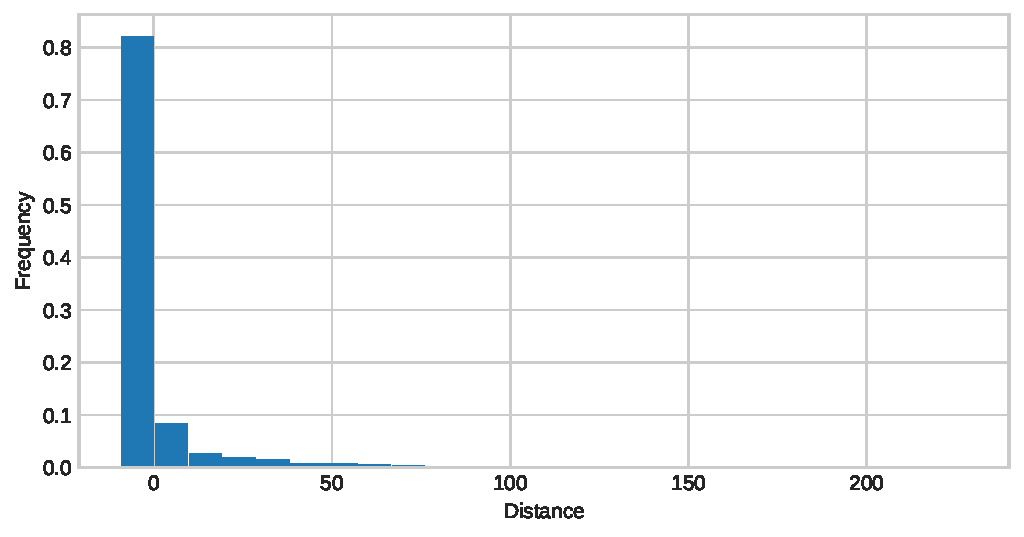
\includegraphics[width=.85\textwidth]{evaluation-results/figures/distance-distribution-histogram-Geometric-25.pdf}
    \caption{Matched segments geometric distance distribution histogram (binning=25)}
    \label{fig:distance-distribution-histogram-Geometric-25}
    \end{figure}

    In the current evaluation, the geometric distance between corpus and parser segments spans from a minimum 0 to maximum 219 characters. The mean distance is 4.99, which is close to the minimum point, with a standard deviation of 14.67, which, in relative terms, indicates an extreme deviation of 2940\%. The skew over 1 indicates a strong asymmetry to the right, and the kurtosis of 43.14 (almost 15 times the threshold of 3) indicates that most of the data, about 80\%, gravitate towards the left, between 0 and slightly over the mean, while the rest of the data point continue into a very long tail to the right. This is depicted in Figure \ref{fig:distance-distribution-histogram-Geometric-25}. 
    
    As appears in Figure \ref{fig:distance-distribution-histogram-Geometric-25}, the data follow a power law distribution \citep{newman2005power}. Here 62\% are not shifted at all and 83\% of the segments are slightly shifted up to 5 characters. There rest (27\%) of the segments are shifted by more than 5 characters. These ratios approximate Patetto's 80-20 distribution law but may as well fit Zipf's law \citep{newman2005power}. In future work, properties of these data should further be analysed, including the distribution fitting, that is selection of the theoretical distribution that fits best to a dataset.
    
    \begin{figure}[!ht]
    \centering
    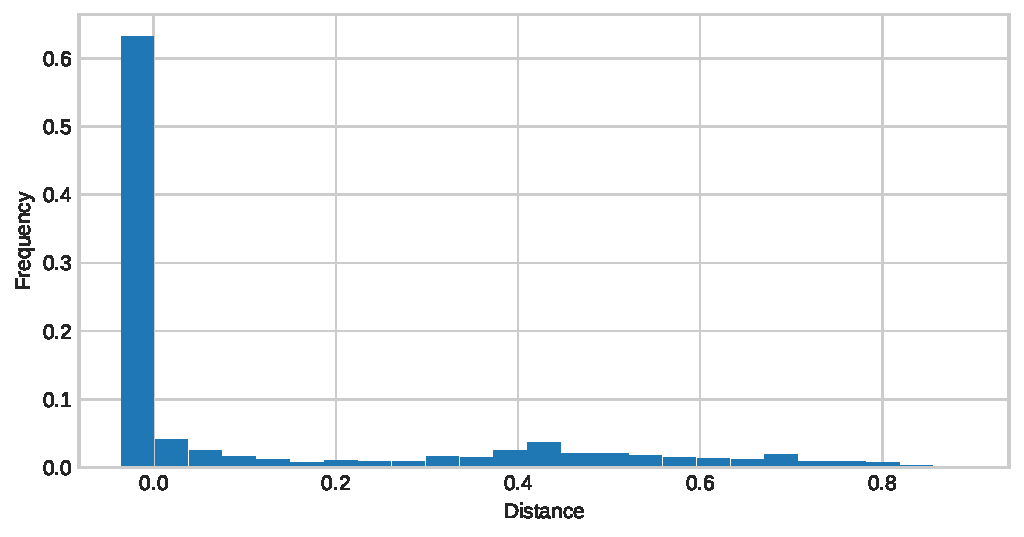
\includegraphics[width=.85\textwidth]{evaluation-results/figures/distance-distribution-histogram-WindowDiff-25.pdf}
    \caption{Matched segments WindowDiff distance distribution histogram (binning=25)}
    \label{fig:distance-distribution-histogram-WindowDiff-25}
    \end{figure}
    
    Next distance that I discuss is WindowDiff distance between corpus and parser segments. One crucial difference to geometric distance is the normalisation to [0,1] interval. In the current evaluation, the WindowDiff distance distribution, depicted in Figure \ref{fig:distance-distribution-histogram-WindowDiff-25}, spans from a minimum 0 to maximum score of 0.86. The mean distance is 0.15 with a standard deviation of 0.23 i.e. $\pm$159\%. The mean value is close to the minimum point, the relative standard deviation indicated extreme deviations of 159\%, the skew over 1 indicates a strong asymmetry to the right, and the kurtosis of 0.28 indicate the distribution does not have many outliers in the tail. 
    
    One positive aspect of this distance distribution is that the tail is not so long due to its normalised structure. This permits aggregation of the outliers we have observed in geometric distance distribution into a compact spectrum. This way, kurtosis, which, in this case, is smaller than 3, no longer indicates an abnormally long tail of outliers. 
    
    The histogram in Figure \ref{fig:distance-distribution-histogram-WindowDiff-25} resembles a power law distribution and more analysis work needs to be done in the future, including the distribution fitting and relation to the causes of partial matches in the first place. 
    
    This section presented the segmentation evaluation and distance analysis of the partially matching segments. The data show that the parser generates segments exactly as provided in the corpus with an accuracy of 0.71, and segments that partially correspond to those in the corpus with an accuracy of 0.8. We will see in the next sections that this partial match is supported by the identical labels that the segments carry. The distances of the partially matched segments, in about 80\% of the cases do not exceed 5 characters, but can span, most probably by mistake, over 200 characters. Next I move on to present the evaluation of the segment label assignments, which in our case are unit classes and functions.

\subsection{Unit class evaluation}
\label{sec:unit-class-evaluation}
    In this and the next section I present the parser syntactic accuracy. The syntactic accuracy aims to measure how well the main unit types and the clause main elements have been detected by the parser compared to the corpus. The evaluation is performed on the OCD corpus. This evaluation is restricted to the clause and four group types: nominal, prepositional, adverbial and adjectival. No clause complexes, group complexes or word types are included. The evaluation data are depicted in Figure \ref{fig:unit-types-data}. The names of the unit classes are provided on the x axis at the bottom of the graph while on the y axis the absolute number of occurrences is provided. 
    
    The meaning of exact and close match has been explained in Section \ref{sec:segmentation-evaluation} and from now on the label ``Matched'' will mean the segments that are either exactly or closely matched all together, while the label with a remark ``(exact only)'' means that it applies to only the portion of the exactly matched segments. 
    
    
    \begin{figure}[!ht]
    \centering
    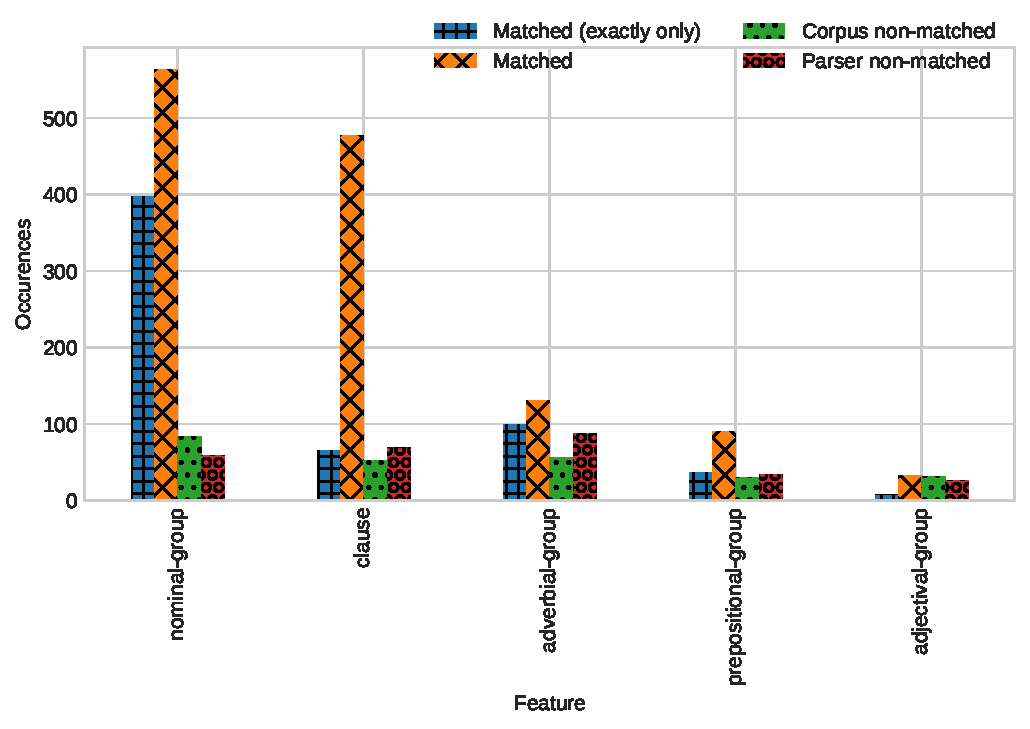
\includegraphics[width=.85\textwidth]{evaluation-results/figures/unit-types-data.pdf}
    \caption{Bar chart of matched and non-matched segments for the main unit classes}
    \label{fig:unit-types-data}
    \end{figure}
    
    To make the data easier to read and interpret I present the evaluation data in a table form using relative values to the number of matched segments. The absolute values of the evaluation statistics are contained in the graphical form and also available in the appendices in the table form. The relative evaluation data in this and the following sections will be presented in tables with the same structure. Using Table \ref{tab:unit-types-relative} as example, the column meaning is as follows. The first column contains the name of the unit class, element or feature. The column ``Matched'' contains the absolute number of matched segments with a specific label. The three other columns represent the number of segments relative to the ``Matched'' ones. So the column ``(\%) Matched (exactly only)'' means that out of all the matched segments that many represent exact matches and the rest to 100\% are partially matched segments. The column ``(\%) Corpus non-matched'' represent the number of segments relative to the total number of segments of particular type in the corpus, which remain unmatched. The column signifies the fraction of segments that remain unmatched, while the rest up to 100\% have, each, a corresponded in the parser output. The column ``(\%) Parser non-matched'' represents the number of segments (relative to the total number of segments of particular type in the parser output) in the parser output that do not have a correspondent in the corpus.
    
    \begin{table}[!ht]
    \centering
    \begin{tabulary}{\textwidth}{lCCCC}
    \toprule
    {} &  Matched &  (\%) Matched (exactly only) &  (\%) Corpus non-matched &  (\%) Parser non-matched \\
    \midrule
    nominal-group       &   564.00 &                       70.39 &                   12.96 &                    9.47 \\
    clause              &   477.00 &                       13.84 &                    9.83 &                   12.64 \\
    adverbial-group     &   131.00 &                       76.34 &                   29.95 &                   40.18 \\
    prepositional-group &    90.00 &                       41.11 &                   25.00 &                   27.42 \\
    adjectival-group    &    33.00 &                       24.24 &                   49.23 &                   44.07 \\
    \bottomrule
    \end{tabulary}
    \caption{The evaluation statistics relative to the number of matched segments for the main unit classes}
    \label{tab:unit-types-relative}
    \end{table}
    
    The evaluation data from Table \ref{tab:unit-types-relative} indicate that most (over 70\%) of the nominal and adverbial groups are identified with exact same borders as in the corpus while clause borders exhibit the most disagreement reflected by their low score of exact matches, only 13.84\%. The proportion of unmatched unit class segments in both the corpus and parser output varies between 9\% for clauses and nominal groups, and over 40\% for adjectival and adverbial groups. These proportions, however, are better interpreted when they are embedded into precision and recall score, which are provided in Table \ref{tab:unit-types-combined-F1}. 
    
    \begin{table}[!ht]
    \centering
    \begin{tabular}{lccc}
    \toprule
    {} &  Precision &  Recall &   F1 \\
    \midrule
    nominal-group       &       0.91 &    0.87 & 0.89 \\
    clause              &       0.87 &    0.90 & 0.89 \\
    prepositional-group &       0.73 &    0.75 & 0.74 \\
    adverbial-group     &       0.60 &    0.70 & 0.65 \\
    adjectival-group    &       0.56 &    0.51 & 0.53 \\
    \bottomrule
    \end{tabular}
    \caption{Parser accuracy statistics for for the main unit classes}
    \label{tab:unit-types-combined-F1}
    \end{table}
    
    Table \ref{tab:unit-types-combined-F1} shows that clause and normal group units are identified with almost 0.9 $F_1$ measure, which is an encouraging result, while the adjectival and adverbial groups score 0.53 and 0.65 indicates that there is some space for improvement. 
    Further investigation is needed to discover the reason for the lower scores as there seem to be no obvious cause other than corpus and/or parser errors. Also, as visible in Figure \ref{fig:unit-types-data}, there is also a contrast in the number of segments between the first two unit types and the last three with a ratio of one to four or more. The low number of exemplars in this evaluation contributes probably to the lower accuracy.
    
\subsection{Unit element evaluation}
\label{sec:unit-element-evaluation}

    


